\chapter{LGR variations} %This title needs fixing

\section{Smaller Cavity LGR} \label{smallLGR}

To achieve stronger MW driving, we also designed and fabricated
smaller LGR with central loop radius $r_c = 2.5$ mm and $n = 4$ outer loops of radius $r_o = 2.45mm$, as shown in Figure \ref{smallLGRfigure}. The naked air-gapped LGR cavity exhibits $f_0 = 4.5$ GHz, similar to the larger LGR design described in the main text. Employing the same exciter antenna, we measure $B_1 = 5.8$ gauss at the center of the smaller LGR device; the measured 3dB bandwidth $\Delta_{3dB} = 112$ MHz corresponds to a loaded quality factor of $Q_L = 25.4$, and an associated ring-down time of 2.8 ns.

\begin{figure}[t!]
\centering
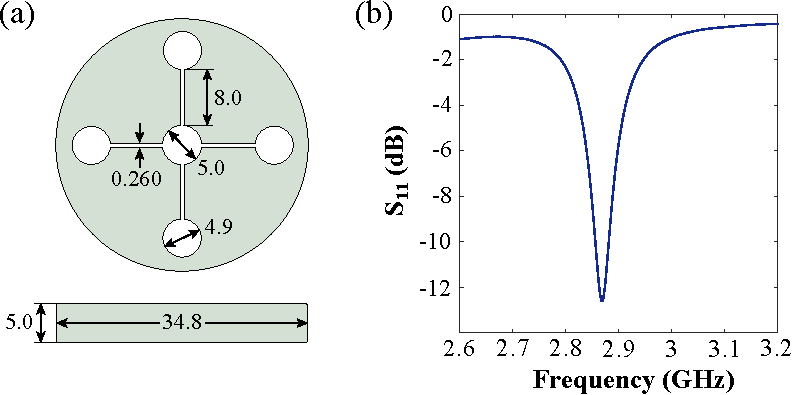
\includegraphics[width = \textwidth]{Figure_B_3.pdf}  
\caption{\textbf{Smaller LGR design} \textbf{(a)} Line drawing of smaller LGR with central loop radius $r_c = 2.5$ mm as described in section \ref{smallLGR}. Units are in mm. \textbf{(b)} Measured $S_{11}$ for composite device tuned to $f_0 \approx 2.87 GHz$.}
\label{smallLGRfigure}
\end{figure}    


\section{Copper LGR}

Copper LGR section.

\clearpage
\newpage
